%%%%%%%%%%%%%%%%%%%%%%%%%%%%%%%%%%%%%%%%%%%%%%%%%%%%%%%%%%%%%%%%%%%%%%%%%%%%%%%%%%%%%%%%%%
%
% TeX file rotcurve-pgm.tex
% Uses: tikz package
% Last Updated:  2023.10.21
% First Created: 2023.10.21
%
% Title: Rotation curve PGM
%
% Description: Draw probabilistic graphical model for the Milky Way rotation curve modelling
%
%%%%%%%%%%%%%%%%%%%%%%%%%%%%%%%%%%%%%%%%%%%%%%%%%%%%%%%%%%%%%%%%%%%%%%%%%%%%%%%%%%%%%%%%%%

\documentclass{article}

\usepackage{times, layouts, xfp}
\usepackage{tikz, hyperref, amsmath, macros-agabrown}
\usetikzlibrary{arrows,shapes,calc,decorations.text}
\usetikzlibrary{backgrounds,patterns,fadings,shadows}
\usepackage{geometry}
\geometry{hmargin=5pt,vmargin=5pt}

\newcommand\showpage{%
\setlayoutscale{0.5}\setlabelfont{\tiny}\printheadingsfalse\printparametersfalse
\currentpage\pagedesign}

\hypersetup{pdftitle={Rotation curve PGM}, pdfsubject={Draw probabilistic graphical model for the Milky Way rotation curve modelling}, pdfauthor=Anthony Brown}

\xdefinecolor{mptab10blue}{rgb}{0.12156862745098039, 0.4666666666666667, 0.7058823529411765}
\xdefinecolor{mptab10orange}{rgb}{1.0, 0.4980392156862745, 0.054901960784313725}
\xdefinecolor{mptab10green}{rgb}{0.17254901960784313, 0.6274509803921569, 0.17254901960784313}
\xdefinecolor{mptab10red}{rgb}{0.8392156862745098, 0.15294117647058825, 0.1568627450980392}
\xdefinecolor{mptab10purple}{rgb}{0.5803921568627451, 0.403921568627451, 0.7411764705882353}
\xdefinecolor{mptab10brown}{rgb}{0.5490196078431373, 0.33725490196078434, 0.29411764705882354}
\xdefinecolor{mptab10magenta}{rgb}{0.8901960784313725, 0.4666666666666667, 0.7607843137254902}
\xdefinecolor{mptab10grey}{rgb}{0.4980392156862745, 0.4980392156862745, 0.4980392156862745}
\xdefinecolor{mptab10olive}{rgb}{0.7372549019607844, 0.7411764705882353, 0.13333333333333333}
\xdefinecolor{mptab10cyan}{rgb}{0.09019607843137255, 0.7450980392156863, 0.8117647058823529}

\tikzstyle{flow}=[->, shorten >=2pt, shorten <=2pt, >=stealth', thick, color=black]
\tikzstyle{flowboth}=[<->, shorten >=2pt, shorten <=2pt, >=stealth', thick, color=black]
\tikzstyle{flow0}=[->, shorten >=0pt, shorten <=0pt, >=stealth', thick, color=black]
\tikzstyle{flowboth0}=[<->, shorten >=0pt, shorten <=0pt, >=stealth', thick, color=black]

\tikzstyle{sampled}=[shape=circle, draw=black, thick, minimum size=1.5cm]
\tikzstyle{fixed}=[shape=circle, fill=black, minimum size=3mm, inner sep=0pt]
\tikzstyle{observed}=[shape=circle, draw=black, fill=black!40!white, thick, minimum size=1.5cm]

\begin{document}
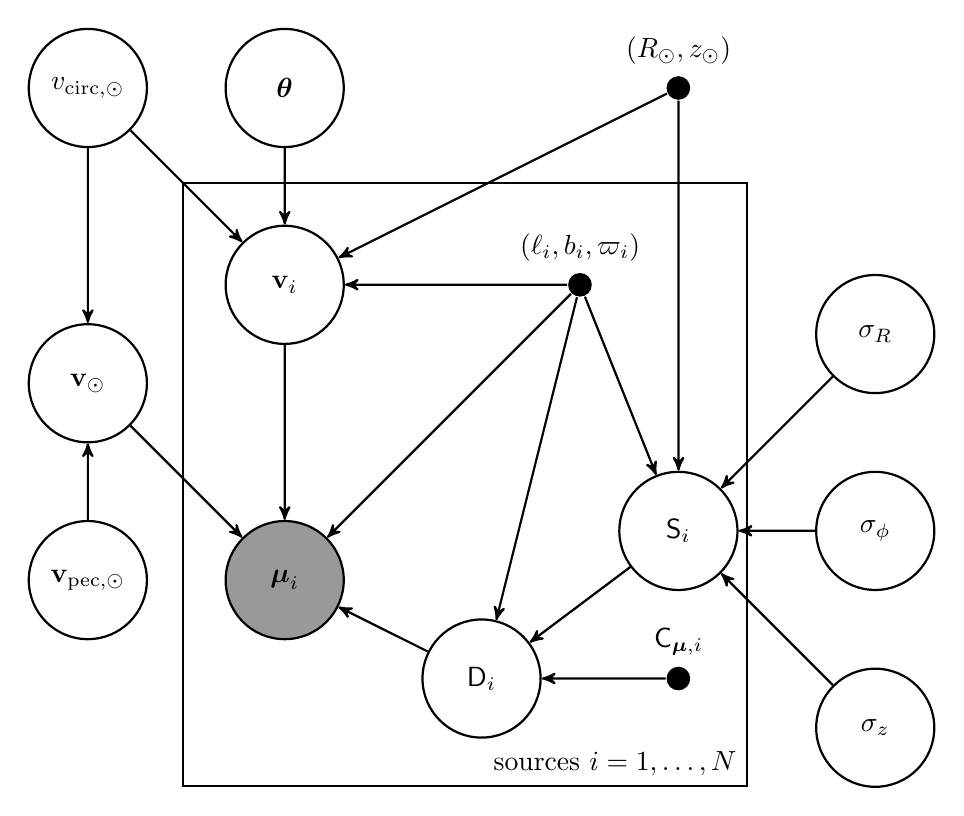
\begin{tikzpicture}[scale=2.5, every path/.style=flow0]
    \node[observed] (pmobs) at (1.5,1.5) {$\boldsymbol{\mu}_i$};
    \node[sampled] (dcov) at (2.5,1.0) {$\mathsf{D}_i$};
    \node[fixed] (covpm) at (3.5,1.0) [label={$\mathsf{C}_{\boldsymbol{\mu},i}$}] {};
    \node[sampled] (vstar) at (1.5,3) {$\mathbf{v}_i$};
    \node[fixed] (posplx) at (3,3) [label={$(\ell_i, b_i, \varpi_i)$}] {};
    \node[sampled] (scov) at (3.5,1.75) {$\mathsf{S}_i$};
    \node[sampled] (vcircsun) at (0.5,4) {$v_{\mathrm{circ},\odot}$};
    \node[sampled] (vsun) at (0.5,2.5) {$\mathbf{v}_\odot$};
    \node[sampled] (theta) at (1.5,4) {$\boldsymbol{\theta}$};
    \node[fixed] (rzsun) at (3.5,4) [label={$(R_\odot, z_\odot)$}] {};
    \node[sampled] (vpecsun) at (0.5,1.5) {$\mathbf{v}_{\mathrm{pec},\odot}$};
    \node[sampled] (sigmar) at (4.5,2.75) {$\sigma_R$};
    \node[sampled] (sigmaphi) at(4.5,1.75) {$\sigma_\phi$};
    \node[sampled] (sigmaz) at (4.5, 0.75) {$\sigma_z$};

    \draw ($(vstar.north west)+(-0.3,0.3)$) rectangle ($(covpm.south east)+(0.3,-0.5)$) node[above left]{sources $i=1,\ldots, N$};

    \draw (dcov) -- (pmobs);
    \draw (covpm) -- (dcov);
    \draw (vstar) -- (pmobs);
    \draw (posplx) -- (vstar);
    \draw (posplx) -- (scov);
    \draw (posplx) -- (dcov);
    \draw (posplx) -- (pmobs);
    \draw (scov) -- (dcov);
    \draw (rzsun) -- (vstar);
    \draw (rzsun) -- (scov);
    \draw (sigmar) -- (scov);
    \draw (sigmaphi) -- (scov);
    \draw (sigmaz) -- (scov);
    \draw (vcircsun) -- (vstar);
    \draw (theta) -- (vstar);
    \draw (vcircsun) -- (vsun);
    \draw (vsun) -- (pmobs);
    \draw (vpecsun) -- (vsun);
\end{tikzpicture}
\end{document}
